\section{Results}
\label{sec:results}

\subsection{Manual cross-validation}
\label{subsec:results-crossval}
Of the \textcolor{red}{30 authors sampled across two waves} under the scheme described in Subsection~\ref{subsec:methods-crossval}, Table~\ref{tab:crossval} summarizes agreement between OpenAlex's \texttt{h\_index} and the corresponding value I located by hand in Web of Science, Scopus, and Google Scholar. Coverage itself varies sharply: Scopus returned a value for \textcolor{red}{26 of the 30 authors}, Google Scholar for \textcolor{red}{19}, and Web of Science for \textcolor{red}{16}.

\begin{table}[h]
	\centering
	\caption{Agreement between OpenAlex and each external source, over authors for which that source returned a value. Diff is OpenAlex minus the external value.}
	\label{tab:crossval}
	\begin{tabular}{@{}lcccc@{}}
	\toprule
	Source & $n$ & Mean diff & Mean abs.\ diff & Worst case \\
	\midrule
	Web of Science & \textcolor{red}{16/30} & $\textcolor{red}{+24.5}$ & \textcolor{red}{25.7} & Lei Jiang ($+100$) \\
	Scopus         & \textcolor{red}{26/30} & $\textcolor{red}{+8.0}$  & \textcolor{red}{12.4} & Donald Small ($+46$) \\
	Google Scholar & \textcolor{red}{19/30} & $\textcolor{red}{-22.7}$ & \textcolor{red}{30.7} & A. Jafari ($-85$) \\
	\bottomrule
	\end{tabular}
\end{table}

Scopus tracks OpenAlex most closely, both in coverage and in magnitude of disagreement. Google Scholar is systematically higher than OpenAlex, consistent with its broader crawl of preprints, theses, and other grey literature and its comparative permissiveness toward self-citation; this ordering (Google Scholar $>$ Scopus $>$ OpenAlex $>$ Web of Science) reproduces cleanly among the \textcolor{red}{six} global top-h\textsubscript{1} sanity-check authors, none of whom show a discrepancy exceeding 27\% of their OpenAlex value in either direction.

Four authors, however, show disagreement well outside this range. I read this as a signature of author-disambiguation failure (multiple distinct people merged under one OpenAlex author ID) rather than of genuine cross-database disagreement:
\begin{itemize}
	\item \textbf{Donald Small} (Johns Hopkins): $\mathrm{h}_1^{\mathrm{OpenAlex}}=103$ against Scopus $=57$ and Google Scholar $=59$.
	\item \textbf{Karen S.\ Calhoun} (University of Michigan): $\mathrm{h}_1^{\mathrm{OpenAlex}}=45$ against Scopus $=11$ and Google Scholar $=13$.
	\item \textbf{Lei Jiang} (University of Science and Technology of China): $\mathrm{h}_1^{\mathrm{OpenAlex}}=215$ against Web of Science $=115$, consistent with documented China-specific coverage discrepancies in OpenAlex~\citep{zheng2025}.
	\item \textbf{A.\ Jafari} (Sharif University of Technology): $\mathrm{h}_1^{\mathrm{OpenAlex}}=139$, but Web of Science, Scopus, and Google Scholar report $41$, $133$, and $224$ respectively.
\end{itemize}
All four fall in the non-Anglophone-institution or common-name strata of the sample, matching the concern raised in Subsection~\ref{subsec:methods-crossval} that disambiguation is more error-prone for exactly these authors. Because such merges can only inflate an author's apparent $\mathrm{h}_1$, and $\mathrm{h}_1$ feeds directly into $\mathrm{h}_2$ and $\mathrm{h}_3$, a handful of merged identities at the right institution could measurably distort an institution- or country-level ranking; I flag this as an open limitation rather than one this sample can size definitively. \textcolor{red}{This sample is deliberately adversarial, chosen to find errors, not to estimate how often they occur. The 4/30 (13\%) outlier fraction should not be read as an estimate of how much of the full dataset is affected. The same pattern, disambiguation precision concentrated lower for common names and non-Anglophone institutions, appears in an independent benchmark of 2{,}700 scholars sampled systematically across three regions~\citep{zhao2025}, corroborating that this is a geographically and onomastically concentrated failure mode rather than an artifact of this particular sample. OpenAlex's maintainers report an ongoing correction effort targeting exactly this kind of over-merging, with corresponding-author identification precision rising from 0.60 to 0.92 (F1 0.72 to 0.90) after a 2026 rework of the underlying author-matching model~\citep{demes2026}. Subsection~\ref{subsec:results-sensitivity} quantifies how much a population-wide error rate at or below the adversarial sample's raw rate would actually move this paper's rankings.}

\textcolor{red}{The four Arts and Humanities threshold authors sampled (Gillian Ramchand and G.\ Herbert Fowler at Oxford; D.H.\ Mellor and James Raven at Cambridge) illustrate the range of under-coverage across major citation databases: Ramchand and Fowler returned no value in any of the three external sources, while Mellor (OA~$\mathrm{h}_1=28$) and Raven (OA~$\mathrm{h}_1=24$) appeared in Scopus at roughly half their OpenAlex values ($\mathrm{h}_1=13$ and 12, respectively); for Raven, Google Scholar (26) brackets the OpenAlex value closely.} This is consistent with the well-documented weaker coverage of book-based humanities scholarship in all major citation databases~\citep{nederhof2006} and suggests that h-index comparisons in these fields should be read with correspondingly less confidence than in the sciences.

\subsection{The overall h\textsubscript{2} ranking}
\label{subsec:overall-h2}
Table~\ref{tab:overall-h2} lists the ten institutions with the highest institution-level h\textsubscript{2}, computed over all 20,932 institutions and 30.0 million authors described in Section~\ref{sec:methodology}.

\begin{table}[h]
	\centering
	\caption{Top 10 institutions by overall h\textsubscript{2}.}
	\label{tab:overall-h2}
	\begin{tabular}{@{}lrr@{}}
	\toprule
	Institution & h\textsubscript{2} & Authors \\
	\midrule
	Harvard University & 137 & 110,979 \\
	Stanford University & 107 & 65,197 \\
	University of Cambridge & 105 & 52,307 \\
	Cornell University & 104 & 70,718 \\
	Johns Hopkins University & 103 & 80,028 \\
	University of Oxford & 103 & 57,110 \\
	University of Washington & 102 & 71,270 \\
	University of North Carolina at Chapel Hill & 101 & 64,478 \\
	University College London & 100 & 77,482 \\
	University of California, San Francisco & 100 & 50,351 \\
	\bottomrule
	\end{tabular}
\end{table}

This broadly tracks the US News and World Report ranking, where Harvard also places 1st, Stanford 3rd, and Cambridge 5th. As I show below, however, the overall ranking is a considerably less interesting object than it first appears.

\subsection{Field-level heterogeneity}
\label{subsec:field-level}
Splitting h\textsubscript{2} by (institution, field) reveals that the overall ranking is deceptive: several institutions that never come close to the top of Table~\ref{tab:overall-h2} \textcolor{red}{rank first globally in their field by this measure}. Table~\ref{tab:field-leaders} lists a sample of these cases.

\begin{table}[h]
	\centering
	\small
	\caption{Selected field leaders that rank well outside the overall top 10. ``Overall'' columns give the institution's rank and h\textsubscript{2} in Table~\ref{tab:overall-h2}'s full ranking; ``Field h\textsubscript{2}'' is the institution's h\textsubscript{2} restricted to that field.}
	\label{tab:field-leaders}
	\renewcommand{\arraystretch}{1.2}
	\begin{tabular}{@{}>{\raggedright\arraybackslash}p{2.5cm}>{\raggedright\arraybackslash}p{3.4cm}rrr@{}}
	\toprule
	Field & Leader & Ov.\ rank & Ov.\ h\textsubscript{2} & Field h\textsubscript{2} \\
	\midrule
	Agricultural \& Biological Sciences & Wageningen & 172 & 71 & 56 \\
	Environmental Science & Wageningen & 172 & 71 & 56 \\
	Pharmacology, Toxicology \& Pharmaceutics & Shenyang Pharmaceutical University & 535 & 53 & 24 \\
	Computer Science & Carnegie Mellon University & 175 & 70 & 56 \\
	Materials Science & USTC & 39 & 89 & 59 \\
	Engineering & USTC & 39 & 89 & 62 \\
	Energy & USTC & 39 & 89 & 52 \\
	Chemical Engineering & Univ.\ of Chinese Academy of Sciences & 91 & 80 & 23 \\
	Dentistry & Universidade de São Paulo & 235 & 66 & 34 \\
	\bottomrule
	\end{tabular}
	\renewcommand{\arraystretch}{1}
\end{table}

University of Antwerp is the counterexample that proves the rule holds both ways: it is \#14 overall ($\mathrm{h}_2=98$) \emph{and} \#1 in Physics and Astronomy ($\mathrm{h}_2=96$), a broad powerhouse that also \textcolor{red}{ranks first in} a specific, non-biomedical field. Universidade Estadual de Campinas (UNICAMP) places 6th in Dentistry behind São Paulo, \textcolor{red}{placing Brazil among the top six globally in Dentistry by this measure} despite the country appearing nowhere near the top of any general-purpose ranking~\citep{vaccaro2022bibliometrics}. China's cluster is not one specialty but four related applied-science fields: University of Science and Technology of China (USTC) \textcolor{red}{ranks first in} Materials Science, Engineering, and Energy \textcolor{red}{by field h\textsubscript{2}}, while its sister institution, the University of Chinese Academy of Sciences, \textcolor{red}{ranks first in} Chemical Engineering.

Not every field supports this kind of comparison equally well. Decision Sciences is the thinnest field in the dataset: Stanford's global \#1 is $\mathrm{h}_2=22$, built on only 285 Stanford authors against 140,147 authors field-wide, versus Medicine's $\mathrm{h}_2=119$ built on 7.58 million authors field-wide. h\textsubscript{2} is not meaningfully comparable across fields of such different size, only within a field, and Decision Sciences in particular may be too sparse an OpenAlex topic category for its ranking to carry much signal.

\subsection{\textcolor{red}{Robustness of field-specific rankings to multi-field assignment}}
\label{subsec:results-field-robustness}
\textcolor{red}{The single-field assignment described in Subsection~\ref{subsec:author-assignment} asks which field accounts for the plurality of an author's publication volume, and assigns them exclusively there. To test how much this choice moves the field-level rankings, I re-run the field-specific h\textsubscript{2} computation after allowing each author to count in every field for which their OpenAlex topic-weight share is at least $\tau$ in accordance with Subsection~\ref{subsec:methods-field-robustness}.}

\textcolor{red}{At $\tau = 33\%$ (an author must contribute at least one third of their output to count in a field), the (institution, field) pair count rises by 9.3\% (333{,}132 $\to$ 364{,}032 pairs). The Spearman rank correlation between original and multi-field h\textsubscript{2} values, computed on the inner join of shared pairs, is $\rho = 0.963$: field rankings are highly stable. Of the 27 fields' leading institutions, 23 are unchanged. The Wageningen Ag\&Bio leadership (Table~\ref{tab:field-leaders}) survives and Carnegie Mellon's Computer Science lead survives. The one notable exception is Environmental Science: the University of Colorado Boulder overtakes Wageningen at this threshold, because Boulder has a larger body of researchers who do substantial but not modal Environmental Science work. The two methods answer different questions. The single-field assignment identifies institutions where Environmental Science is researchers' \emph{primary} field; the multi-field assignment identifies institutions with the most researchers for whom it is a \emph{substantial} field.}

\textcolor{red}{At $\tau = 20\%$ (a more aggressive threshold admitting all authors with one fifth or more of their output in a field), the pair count rises by 20.7\% and $\rho = 0.907$; 18 of 27 field leaders survive. Carnegie Mellon's Computer Science lead also falls at this threshold, with Stanford leading instead, consistent with the same mechanism of Stanford having a larger population of researchers with at least 20\% CS output, even if CS is not their modal field. The Wageningen Ag\&Bio and Environmental Science results are unchanged from the 33\% case. These findings confirm that the overall field ranking structure is broadly stable under multi-field assignment but that the field-leadership claims for smaller, highly specialised institutions depend on how narrowly ``counts in this field'' is defined. Given this sensitivity, the field-leadership claims in Table~\ref{tab:field-leaders} should be read as reflecting depth of specialisation under the paper's single-field assignment.}

\subsection{Concentration within fields}
\label{subsec:gini}
Table~\ref{tab:gini} reports, for every field, the Gini coefficient of institutional h\textsubscript{2} defined in Section~\ref{subsec:methods-supplementary}, together with the field's institution count, leading (maximum) h\textsubscript{2}, and mean h\textsubscript{2}.

\begin{table}[h]
	\centering
	\small
	\caption{Gini coefficient of institutional h\textsubscript{2} within each field, sorted from most to least concentrated.}
	\label{tab:gini}
	\begin{tabular}{@{}lrrrr@{}}
	\toprule
	Field & Institutions & Max h\textsubscript{2} & Mean h\textsubscript{2} & Gini \\
	\midrule
	Physics and Astronomy & 12,739 & 96 & 6.11 & 0.605 \\
	Biochemistry, Genetics \& Molecular Biology & 15,404 & 104 & 6.61 & 0.578 \\
	Neuroscience & 11,646 & 64 & 4.41 & 0.574 \\
	Immunology and Microbiology & 9,838 & 67 & 3.97 & 0.561 \\
	Materials Science & 13,097 & 59 & 6.36 & 0.560 \\
	Earth and Planetary Sciences & 12,447 & 60 & 4.30 & 0.557 \\
	Chemistry & 12,103 & 41 & 5.02 & 0.541 \\
	Environmental Science & 16,603 & 56 & 5.54 & 0.541 \\
	Engineering & 17,742 & 62 & 6.91 & 0.533 \\
	Medicine & 19,119 & 119 & 8.58 & 0.528 \\
	Agricultural and Biological Sciences & 16,391 & 56 & 5.61 & 0.522 \\
	Energy & 8,971 & 52 & 3.38 & 0.515 \\
	Psychology & 15,745 & 58 & 3.64 & 0.513 \\
	Computer Science & 16,736 & 56 & 5.08 & 0.512 \\
	Dentistry & 8,303 & 34 & 3.01 & 0.500 \\
	Mathematics & 11,092 & 36 & 3.42 & 0.491 \\
	Economics, Econometrics and Finance & 13,923 & 55 & 3.30 & 0.482 \\
	Business, Management and Accounting & 14,623 & 32 & 3.59 & 0.481 \\
	Health Professions & 14,840 & 41 & 2.88 & 0.465 \\
	Social Sciences & 19,242 & 48 & 4.57 & 0.461 \\
	Pharmacology, Toxicology and Pharmaceutics & 7,219 & 24 & 2.61 & 0.459 \\
	Chemical Engineering & 5,874 & 23 & 2.48 & 0.446 \\
	Arts and Humanities & 15,390 & 30 & 2.78 & 0.443 \\
	Nursing & 8,958 & 31 & 2.37 & 0.433 \\
	Decision Sciences & 10,409 & 22 & 2.37 & 0.423 \\
	Veterinary & 4,678 & 28 & 2.04 & 0.422 \\
	\bottomrule
	\end{tabular}
\end{table}

Physics and Astronomy is the most unequal field: University of Antwerp's $\mathrm{h}_2=96$ is 15.7 times the field mean of 6.1. Veterinary and Decision Sciences are the most evenly distributed (Gini $\approx 0.42$). Medicine sits in the middle of the table (0.528) despite Harvard's large absolute lead, because Medicine, unlike Physics and Astronomy, has thousands of institutions with meaningful h\textsubscript{2} rather than a single dominant outlier.

\subsection{The overall ranking as an implicit biomedical ranking}
\label{subsec:nonbiomedical}
Medicine alone accounts for 7.58 million of the dataset's 30.0 million authors (25\%), and, together with Biochemistry/Genetics/Molecular Biology, Immunology and Microbiology, Neuroscience, and Health Professions, the five core biomedical fields dwarf every other field's author pool. Table~\ref{tab:nonbio} recomputes institution-level h\textsubscript{2} after excluding authors in these five fields entirely to test whether the overall ranking in Table~\ref{tab:overall-h2} is, in substance, a ranking of medical school size.

\begin{table}[h]
	\centering
	\caption{Top 10 institutions by non-biomedical h\textsubscript{2}, alongside their position in the unrestricted overall ranking. $\Delta$rank is overall rank minus non-biomedical rank; positive means the institution moves up once biomedical fields are excluded.}
	\label{tab:nonbio}
	\begin{tabular}{@{}lrrrrr@{}}
	\toprule
	Institution & Rank & h\textsubscript{2} & Overall rank & Overall h\textsubscript{2} & $\Delta$rank \\
	\midrule
	Harvard University & 1 & 100 & 1 & 137 & 0 \\
	University of Antwerp & 2 & 97 & 14 & 98 & +12 \\
	California Institute of Technology & 3 & 94 & 15 & 97 & +12 \\
	Stanford University & 4 & 92 & 2 & 107 & $-$2 \\
	Université Paris-Saclay & 5 & 91 & 22 & 95 & +17 \\
	Massachusetts Institute of Technology & 6 & 89 & 25 & 94 & +19 \\
	University of Geneva & 7 & 88 & 29 & 93 & +22 \\
	Univ.\ of Science and Technology of China & 8 & 88 & 39 & 89 & +31 \\
	ETH Zurich & 9 & 87 & 36 & 89 & +27 \\
	University of Cambridge & 10 & 87 & 3 & 105 & $-$7 \\
	\bottomrule
	\end{tabular}
\end{table}

Harvard remains \#1 even with its biomedical authors removed, confirming the claim in Subsection~\ref{subsec:field-level} that it is genuinely excellent rather than merely large. But the rest of the table reshuffles substantially: Antwerp, Caltech, Paris-Saclay, MIT, Geneva, USTC, and ETH Zurich all gain 12 to 31 places once Medicine and its four sibling fields are set aside, while Stanford and Cambridge, both anchored by large medical schools, fall by 2 and 7 places respectively. The University of Chinese Academy of Sciences shows the same pattern one tier down: 91st overall but 23rd non-biomedical. Because medical fields have by far the largest, most-cited author pools, they structurally dominate any university-wide aggregate; an institution elite in non-medical fields, such as USTC or Carnegie Mellon, can never reach the top of the overall list no matter how good it is, simply because it lacks a large medical school. The field-level and non-biomedical breakdowns matter more than the unrestricted university-level number.

\subsection{Breadth versus depth}
\label{subsec:breadth}
Table~\ref{tab:field-leaders} showed institutions that lead a single field while sitting far outside the overall top 100. Table~\ref{tab:breadth} shows the opposite pattern: institutions whose strength is broad rather than deep, measured by how many of the 26 fields they place in the global top 50.

\begin{table}[h]
	\centering
	\caption{The nine institutions with the most top-50 field placements out of 26 fields.}
	\label{tab:breadth}
	\begin{tabular}{@{}lrrrr@{}}
	\toprule
	Institution & Top 50 & Top 10 & Overall rank & Overall h\textsubscript{2} \\
	\midrule
	University of California, Los Angeles & 20 & 8 & 13 & 99 \\
	University of Michigan & 20 & 7 & 26 & 94 \\
	Harvard University & 19 & 13 & 1 & 137 \\
	University of Oxford & 19 & 8 & 6 & 103 \\
	University of Washington & 17 & 8 & 7 & 102 \\
	University of Toronto & 17 & 7 & 11 & 100 \\
	Cornell University & 17 & 6 & 4 & 104 \\
	Univ.\ of North Carolina at Chapel Hill & 17 & 5 & 8 & 101 \\
	University of Cambridge & 17 & 4 & 3 & 105 \\
	\bottomrule
	\end{tabular}
\end{table}

UCLA and the University of Michigan share the greatest breadth by this measure, each placing in the global top 50 in 20 of 26 fields; UCLA leads 8 outright while Michigan leads 7. Harvard still leads more fields outright (13 of 26) than any other institution, but four of the nine broadest institutions by this top-50 count, Toronto, UNC Chapel Hill, Washington, and Cambridge, place fewer than half their 17 top-50 fields inside the top 10, meaning most of their breadth comes from being solidly good across many fields rather than dominant in any one. At the other extreme, Boston University (rank 23, $\mathrm{h}_2=94$) achieves its overall strength with zero top-10 field placements, through scale and consistency across many merely-good departments rather than fielding the single best group in any one discipline.

\subsection{Institution efficiency}
\label{subsec:h2-efficiency}

\subsubsection*{Model validation}
Figure~\ref{fig:h2-vs-size} plots institution-level $\mathrm{h}_2$ against the Egghe-predicted value $\mathrm{S}^{1/\beta_1}$ for all institutions with at least 10 OpenAlex authors. A no-intercept regression, appropriate because $N = 0$ authors forces $\mathrm{h}_2 = 0$, gives slope $c = 1.945$ and uncentered $R^2 = 0.911$: $\mathrm{S}^{1/\beta_1}$ alone explains 91\% of the variance in $\mathrm{h}_2$, confirming that Egghe's power-law functional form describes the data. The efficiency metric $\varepsilon_2 = \mathrm{h}_2 / \mathrm{S}^{1/\beta_1}$ captures each institution's deviation from this overall trend.

\begin{figure}[h]
\centering
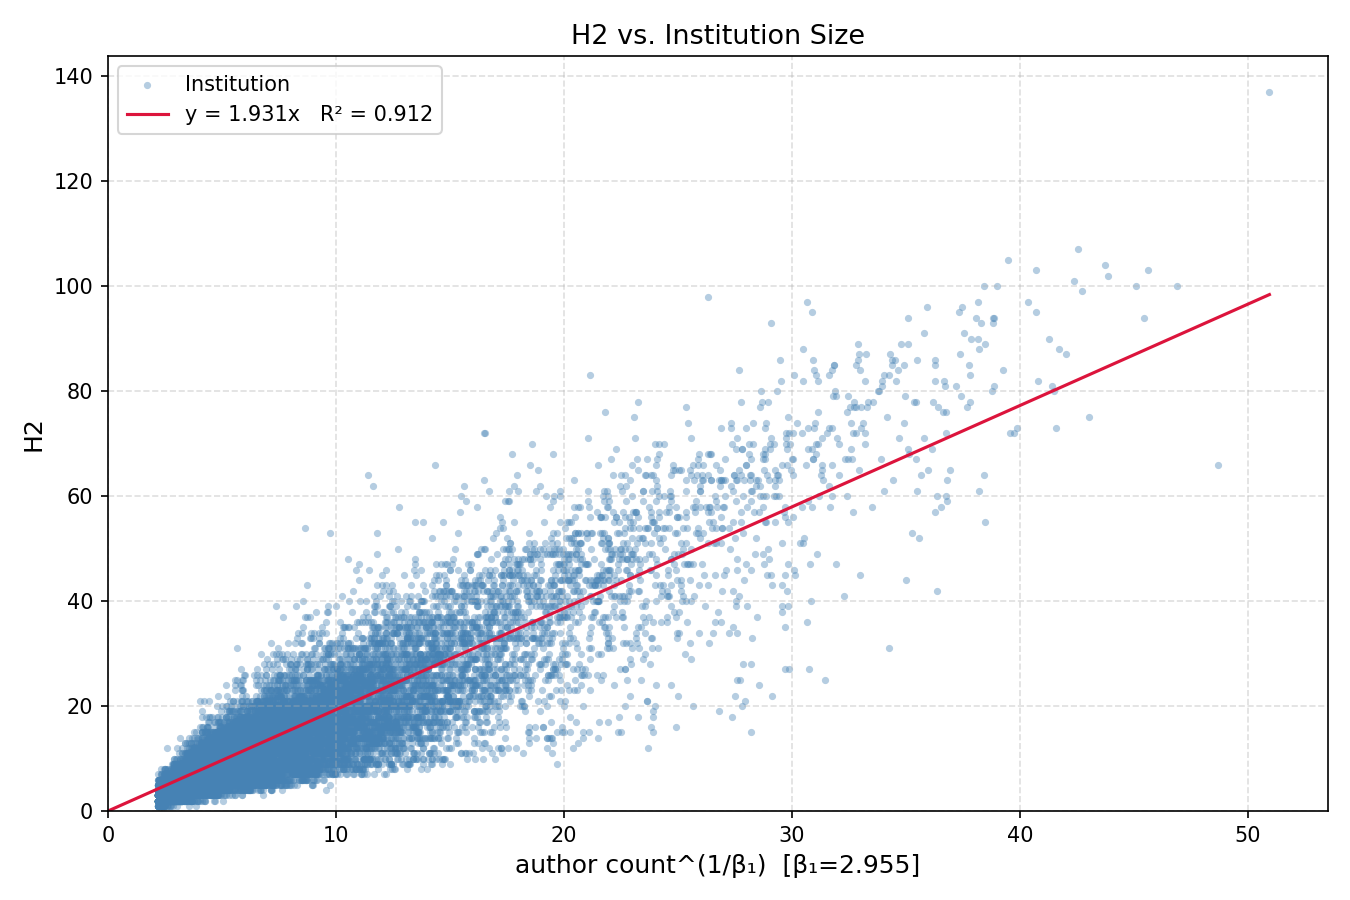
\includegraphics[width=0.85\textwidth]{figures/h2_vs_size.png}
\caption{Institution-level h\textsubscript{2} versus $\mathrm{S}^{1/\beta_1}$ (Egghe's predicted scaling, $\beta_1 = 2.963$). No-intercept regression: $\mathrm{h}_2 = 1.945\,\mathrm{S}^{1/\beta_1}$, $R^2 = 0.911$ (uncentered).}
\label{fig:h2-vs-size}
\end{figure}

The cross-check on Egghe's compounding structure fails sharply, however. Egghe's derivation requires that the Lotka tail exponent of the h\textsubscript{1} distribution equals the product $\alpha_0 \alpha_1$; these separate fits give $\alpha_0 = 2.742$ and $\alpha_1 = 2.996$, whose product is $8.21$, against the directly-measured $\beta_1 = 2.963$: a discrepancy of $177\%$. The analogous prediction at the next level ($\beta_2 = \beta_1 \alpha_2$) is similarly violated: $2.963 \times 1.994 = 5.909$ against the directly-measured $\beta_2 = 2.998$ ($97\%$ discrepancy).

\textcolor{red}{The failure of the compounding formula does not, however, undermine the efficiency metric. The two claims play different roles. The compounding formula ($\beta_1 = \alpha_0\alpha_1$) is a \emph{theoretical prediction} about the relationship between separately-fitted exponents; it is tested here and found wanting. The power-law scaling $\mathrm{h}_2 \propto \mathrm{S}^{1/\beta_1}$ is an \emph{empirical finding} ($R^2 = 0.911$) that does not depend on the compounding formula being correct. $\beta_1$ is estimated directly from the distribution of $\mathrm{h}_1$ values across authors, not derived from $\alpha_0\alpha_1$, so the 177\% discrepancy in the compounding formula has no bearing on the exponent actually used in $\varepsilon_2$. This can be externally validated against the Leiden Ranking later in this subsection to provide an independent, data-driven confirmation based on the correlation between $\varepsilon_2$ and mean normalised citation score.}

\subsubsection*{Efficiency rankings}
The efficiency metric $\varepsilon_2 = \mathrm{h}_2 / \mathrm{S}^{1/\beta_1}$ addresses Mryglod et al.'s~\citeyearpar{mryglod2022} concern directly: because $\mathrm{S}^{1/\beta_1}$ accounts for 91\% of the variance in $\mathrm{h}_2$, dividing it out isolates the residual variation that is not explained by headcount alone.

Table~\ref{tab:h2-efficiency-all} lists the top 10 institutions by $\varepsilon_2$ among the 12,026 with at least 100 authors. The top of the ranking is dominated by small and highly specialized institutions. Focused research centers and specialized colleges recur throughout the top 20.

\begin{table}[h]
	\centering
	\caption{Top 10 institutions by efficiency $\varepsilon_2 = \mathrm{h}_2 / \mathrm{S}^{1/\beta_1}$ ($\beta_1 = 2.963$) among those with at least 100 authors ($n = 12{,}026$).}
	\label{tab:h2-efficiency-all}
	\begin{tabular}{@{}lrrrr@{}}
	\toprule
	Institution & $\varepsilon_2$ & h\textsubscript{2} & Authors & h\textsubscript{2} rank \\
	\midrule
	Bellevue University                                   & 6.24 & 54 &     590 &    497 \\
	Augustana University                                  & 5.61 & 64 &   1,332 &    264 \\
	Center for Behavioral Brain Sciences                  & 5.48 & 31 &     168 &  1,908 \\
	Barcelona Inst.\ of Science and Technology            & 5.43 & 53 &     839 &    520 \\
	Imperial Valley College                               & 5.33 & 62 &   1,412 &    319 \\
	Saint Camillus International Univ.\ of Health Sci.   & 5.30 & 39 &     364 &  1,228 \\
	City College of San Francisco                         & 4.92 & 43 &     605 &    934 \\
	Frederick Community College                           & 4.81 & 37 &     416 &  1,331 \\
	Acad\'{e}mie Nationale de M\'{e}decine                & 4.72 & 39 &     512 &  1,192 \\
	Natl.\ Interuniversity Consortium of Materials Sci.  & 4.67 & 40 &     571 &  1,150 \\
	\bottomrule
	\end{tabular}
\end{table}

Table~\ref{tab:h2-efficiency} restricts to the 1,339 institutions with at least 5,000 authors. The leading institutions are now a mix of specialized research institutes like Rockefeller University ($\varepsilon_2 = 3.77$, biomedical), the Institute of Cancer Research ($\varepsilon_2 = 3.57$), and the London School of Hygiene \& Tropical Medicine ($\varepsilon_2 = 3.44$) and comprehensive universities like the University of Antwerp ($\varepsilon_2 = 3.72$, $\mathrm{h}_2 = 98$, efficiency rank 112). The University of California System, treated here as a single institution under its OpenAlex identifier, is the only entry in the top 100 on both metrics simultaneously (h\textsubscript{2} rank 73, efficiency rank 67). Among the comprehensive elite research universities that dominate the raw $\mathrm{h}_2$ table, Caltech (efficiency rank 367), the University of Geneva (344), and Université Paris-Saclay (465) are the most efficient, each achieving $\mathrm{h}_2 \geq 93$ with under 25,000 authors.

\begin{table}[h]
	\centering
	\caption{Top 10 institutions by efficiency $\varepsilon_2 = \mathrm{h}_2 / \mathrm{S}^{1/\beta_1}$ ($\beta_1 = 2.963$) among those with at least 5,000 authors ($n = 1{,}339$).}
	\label{tab:h2-efficiency}
	\begin{tabular}{@{}lrrrr@{}}
	\toprule
	Institution & $\varepsilon_2$ & h\textsubscript{2} & Authors & h\textsubscript{2} rank \\
	\midrule
	University of California System              & 3.93 &  83 &   8,242 &   73 \\
	Rockefeller University                       & 3.77 &  70 &   5,637 &  179 \\
	University of Antwerp                        & 3.72 &  98 &  15,759 &   14 \\
	Institute of Cancer Research                 & 3.57 &  66 &   5,570 &  230 \\
	University of San Diego                      & 3.56 &  64 &   5,097 &  286 \\
	California University of Pennsylvania        & 3.49 &  76 &   9,011 &  121 \\
	University of Wuppertal                      & 3.48 &  68 &   6,515 &  209 \\
	London School of Hygiene \& Tropical Medicine & 3.44 &  65 &   5,903 &  249 \\
	Royal Holloway, University of London         & 3.39 &  61 &   5,102 &  339 \\
	Vita-Salute San Raffaele University          & 3.37 &  71 &   8,171 &  171 \\
	\bottomrule
	\end{tabular}
\end{table}

\subsubsection*{\textcolor{red}{External validation against the Leiden Ranking}}
\label{subsubsec:leiden-validation}
\textcolor{red}{Matching the 1,506 Leiden Ranking Open Edition 2024 universities to OpenAlex's dataset yields 1,495 institutions with both an MNCS value and an institution-wide h\textsubscript{2} from OpenAlex. The Spearman rank correlation between raw h\textsubscript{2} and MNCS is $\rho = 0.634$ ($p \approx 6 \times 10^{-170}$); between $\varepsilon_2$ and MNCS it is $\rho = 0.580$ ($p \approx 5 \times 10^{-135}$). The successive h-index hierarchy captures genuine differences in research quality across institutions rather than differences in size alone.}

% \textcolor{red}{The modest gap between the two correlations ($\Delta\rho = -0.054$) is mechanistically expected. MNCS is itself size-independent by construction (it is a mean, not a total), so subtracting the size component via $\varepsilon_2 = \mathrm{h}_2 / \mathrm{S}^{1/\beta_1}$ removes a source of co-variation with MNCS that exists in raw h\textsubscript{2}. That $\varepsilon_2$ still correlates at 0.58 after size removal---retaining 92\% of h\textsubscript{2}'s correlation with MNCS---confirms that the efficiency normalization does not erase the quality signal; it isolates the portion of h\textsubscript{2} that is attributable to research excellence rather than headcount.}

\subsection{h\textsubscript{3}: country level}
\label{subsec:h3-country}
Aggregating institutional h\textsubscript{2} up to the country level via the same rank-based procedure yields h\textsubscript{3}. Table~\ref{tab:h3-country} lists the ten highest-h\textsubscript{3} countries, and Figure~\ref{fig:choropleth} maps h\textsubscript{3} for all 214 countries with at least one qualifying institution.

\begin{table}[h]
	\centering
	\caption{Top 10 countries by h\textsubscript{3}.}
	\label{tab:h3-country}
	\begin{tabular}{@{}lrr@{}}
	\toprule
	Country & h\textsubscript{3} & Institutions \\
	\midrule
	United States & 70 & 4,242 \\
	China & 55 & 1,078 \\
	Germany & 49 & 505 \\
	United Kingdom & 47 & 548 \\
	Japan & 46 & 1,358 \\
	Italy & 45 & 229 \\
	France & 41 & 394 \\
	Spain & 39 & 156 \\
	South Korea & 37 & 358 \\
	Australia & 36 & 120 \\
	\bottomrule
	\end{tabular}
\end{table}

\begin{figure}[h]
	\centering
	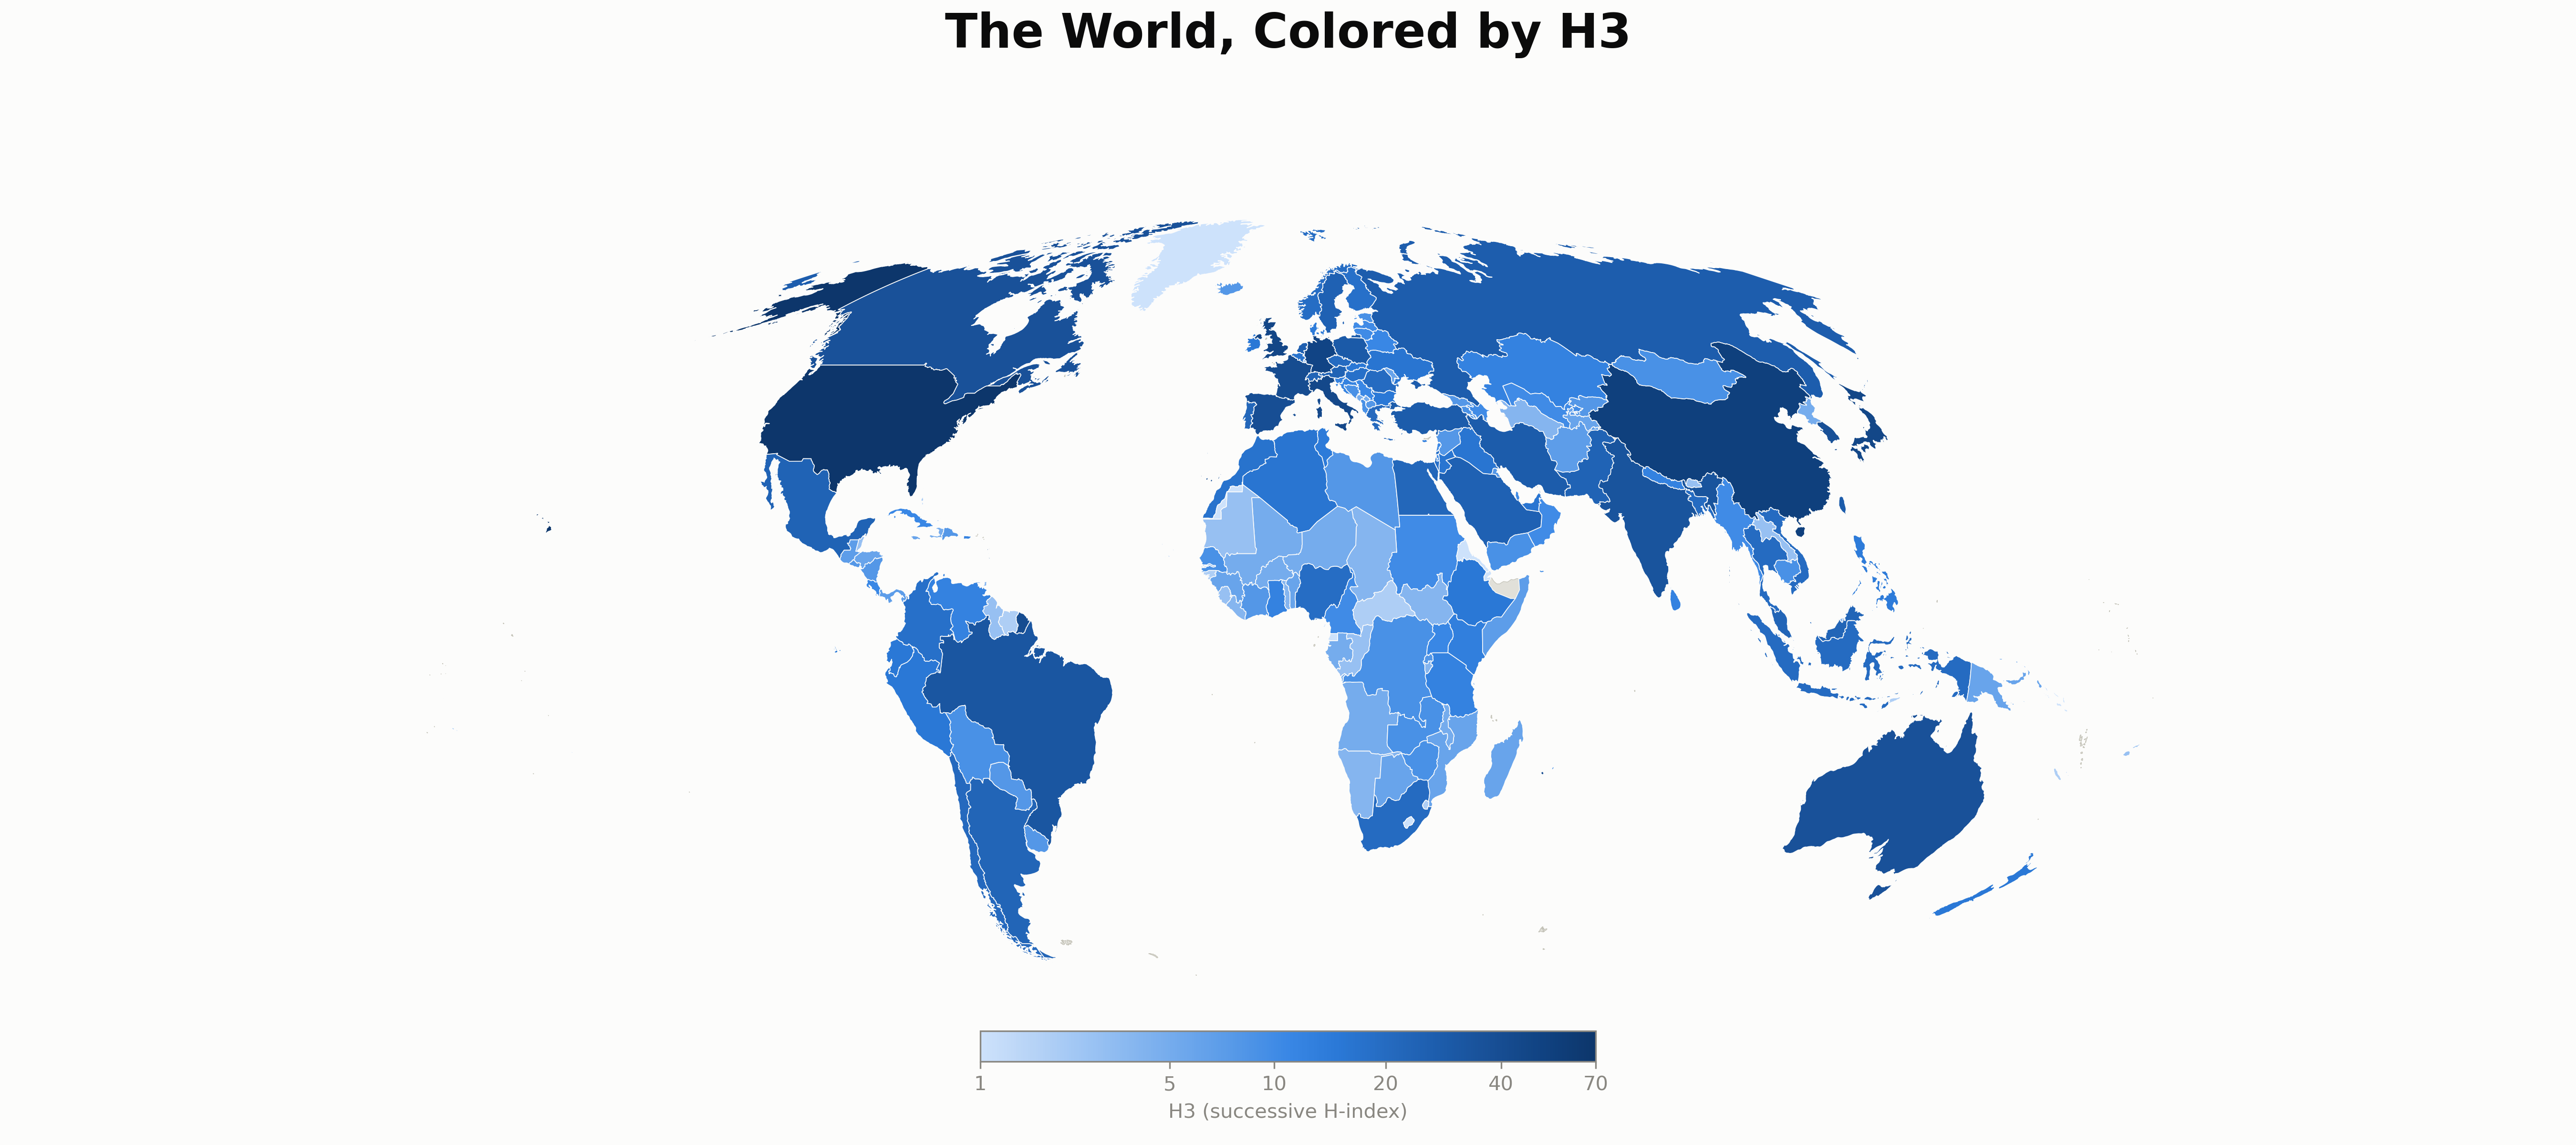
\includegraphics[width=\textwidth]{figures/h3_choropleth.png}
	\caption{h\textsubscript{3} by country. Countries with no qualifying institution are shown in grey.}
	\label{fig:choropleth}
\end{figure}

The United States leads by a wide margin, but Italy's 45 on only 229 institutions and Japan's 46 on 1,358 are a first hint that raw h\textsubscript{3} rewards national research-system size as well as depth, a point to which I return in Subsection~\ref{subsec:h3-efficiency}.

\subsection{Country efficiency}
\label{subsec:h3-efficiency}
Figure~\ref{fig:h3-vs-size} repeats the size-scaling analysis at the country level, plotting $\mathrm{h}_3$ against $\mathrm{R}^{1/\beta_2}$ for each country. The no-intercept fit gives slope $c = 4.064$ and uncentered $R^2 = 0.922$: institution count alone explains 92\% of the variance in $\mathrm{h}_3$ across countries.

\begin{figure}[h]
\centering
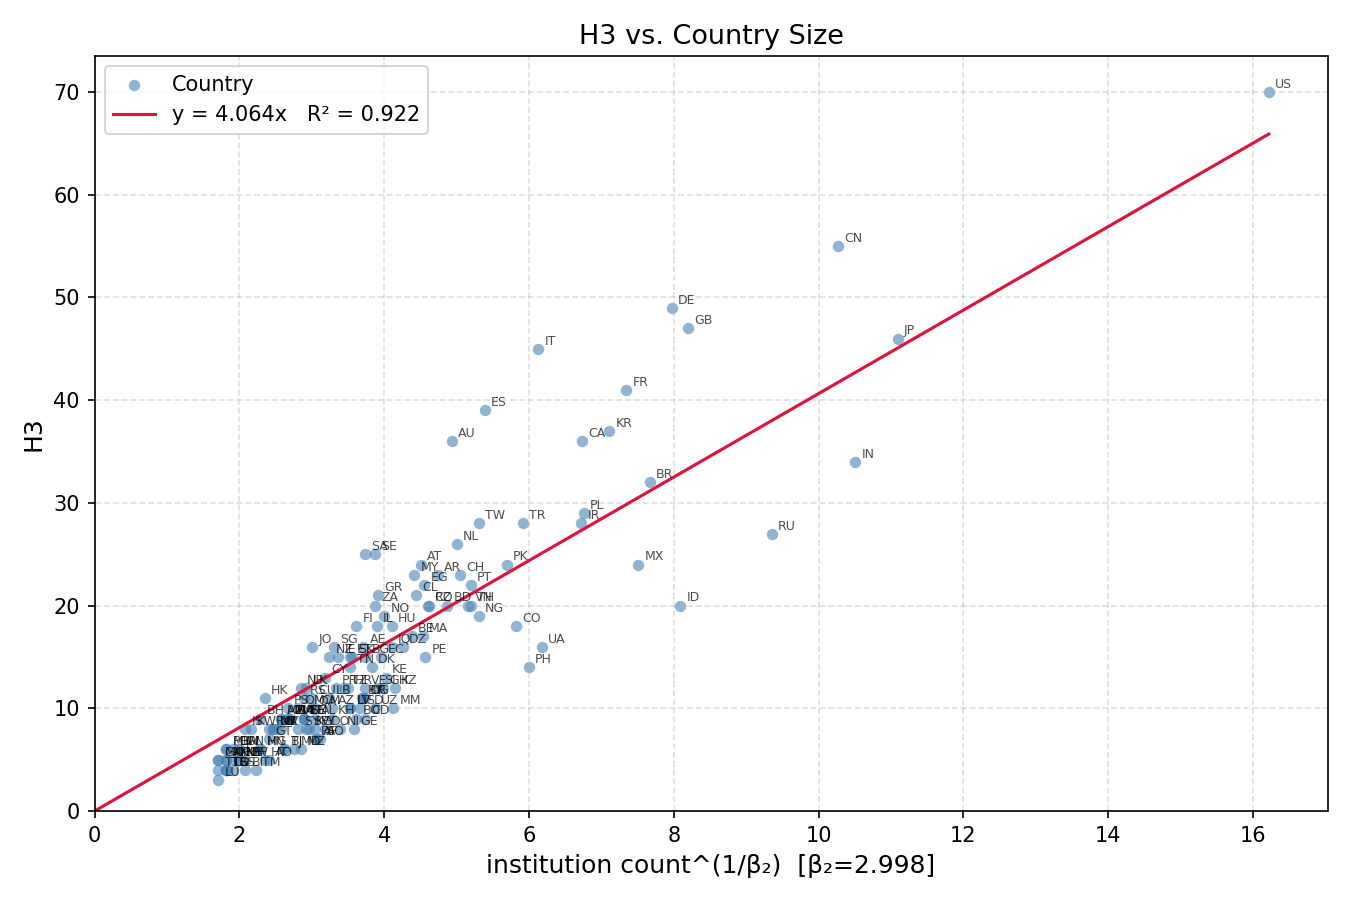
\includegraphics[width=0.85\textwidth]{figures/h3_vs_size.png}
\caption{Country-level h\textsubscript{3} versus $\mathrm{R}^{1/\beta_2}$ (Egghe's predicted scaling, $\beta_2 = 2.998$). No-intercept regression: $\mathrm{h}_3 = 4.064\,R^{1/\beta_2}$, $R^2 = 0.922$ (uncentered).}
\label{fig:h3-vs-size}
\end{figure}

Table~\ref{tab:h3-efficiency} ranks the 151 countries with at least 5 qualifying institutions by efficiency $\varepsilon_3 = \mathrm{h}_3 / \mathrm{R}^{1/\beta_2}$. The Italy--Japan contrast foreshadowed in Subsection~\ref{subsec:h3-country} is now quantified: Italy ($\varepsilon_3 = 7.35$, rank 1) achieves $\mathrm{h}_3 = 45$ from only 229 institutions, while Japan ($\varepsilon_3 = 4.15$, rank 44) reaches $\mathrm{h}_3 = 46$ from 1,358, virtually the same headline number but at $6{\times}$ the institutional scale. Australia (rank 2, $\varepsilon_3 = 7.29$, 120 institutions) and Spain (rank 3, $\varepsilon_3 = 7.24$, 156 institutions) round out a top tier of countries with compact but high-quality research systems. Germany (rank 6), the United Kingdom (rank 7), and France (rank 8) are the only countries that place in the top 10 on both raw $\mathrm{h}_3$ and efficiency, confirming that their research depth is genuine rather than an artefact of institutional scale. Saudi Arabia is a notable outlier at 4th by efficiency (h\textsubscript{3}=25 on just 52 institutions) despite ranking only 20th by raw h\textsubscript{3}; as flagged in Subsection~\ref{subsec:methods-crossval}, this is plausibly an artifact of high-h-index researchers listing Saudi institutions as secondary affiliations in exchange for funding~\citep{saudi} rather than a genuine concentration of resident research talent.

The United States falls to efficiency rank 34 ($\varepsilon_3 = 4.32$) despite its raw lead ($\mathrm{h}_3 = 70$, rank 1). With 4,242 qualifying institutions, nearly $8{\times}$ more than China and $18{\times}$ more than Italy, even a large absolute $\mathrm{h}_3$ advantage is absorbed by the size denominator. China (rank 10, $\varepsilon_3 = 5.36$, 1,078 institutions) is more compact and appears above the US on this metric.% Russia (rank 107, $\varepsilon_3 = 2.89$) and India (rank 83, $\varepsilon_3 = 3.24$) show the converse pattern: large institution counts yielding modest $\mathrm{h}_3$ relative to their scale.

\begin{table}[h]
	\centering
	\caption{Top 10 countries by efficiency $\varepsilon_3 = \mathrm{h}_3 / R^{1/\beta_2}$ ($\beta_2 = 2.998$) among those with at least 5 institutions ($n = 151$).}
	\label{tab:h3-efficiency}
	\begin{tabular}{@{}lrrrr@{}}
	\toprule
	Country & $\varepsilon_3$ & h\textsubscript{3} & Institutions & h\textsubscript{3} rank \\
	\midrule
	Italy          & 7.35 & 45 &    229 &  6 \\
	Australia      & 7.29 & 36 &    120 & 10 \\
	Spain          & 7.24 & 39 &    156 &  8 \\
	Saudi Arabia   & 6.69 & 25 &     52 & 20 \\
	Sweden         & 6.45 & 25 &     58 & 21 \\
	Germany        & 6.14 & 49 &    505 &  3 \\
	United Kingdom & 5.74 & 47 &    548 &  4 \\
	France         & 5.59 & 41 &    394 &  7 \\
	Greece         & 5.36 & 21 &     60 & 31 \\
	China          & 5.36 & 55 &  1,078 &  2 \\
	\bottomrule
	\end{tabular}
\end{table}

\subsection{\textcolor{red}{Sensitivity to disambiguation error}}
\label{subsec:results-sensitivity}
\textcolor{red}{Table~\ref{tab:sensitivity} reports, for six simulated population-wide error rates spanning $p=1\%$ to a deliberately implausible $p=80\%$ (Subsection~\ref{subsec:methods-sensitivity}), the Spearman rank correlation and top-set overlap between the perturbed and unperturbed rankings, averaged over five trials, together with how often the paper's two headline field-leadership claims survive the perturbation intact. The cross-validation sample's own raw outlier fraction (4/30 $\approx 13\%$ across both waves, Subsection~\ref{subsec:results-crossval}) is included as an extra row for reference, though it carries no special status in this analysis.}

\textcolor{red}{Institution- and country-level rank correlations decline only modestly with $p$ and then plateau rather than continuing toward zero: Spearman $\rho$(h\textsubscript{2}) falls from 0.999 at $p=1\%$ to 0.991 at $p=20\%$ and then stays flat at 0.988 all the way out to $p=80\%$; $\rho$(h\textsubscript{3}) shows the same pattern, from 0.9997 down to 0.994. This follows from how h\textsubscript{2} and h\textsubscript{3} are computed: each is an order statistic (the largest rank whose value has not yet fallen below it), so what matters for a given institution or country is whether a noisy author sits near \emph{its own} threshold, not how many noisy authors exist elsewhere in the dataset; and because the perturbation is bounded in magnitude (at most $\approx 4\times$, the largest of the four observed ratios) and applied independently and identically everywhere, raising $p$ further increasingly inflates competing institutions' threshold authors by similar amounts, which cancels out much of the relative shift.}

\textcolor{red}{The field-specific leadership claims for Wageningen (Agricultural \& Biological Sciences, Environmental Science) and Carnegie Mellon (Computer Science) are noisier with five trials per rate: each survives in 3 to 5 of 5 trials at every rate tested. Wageningen's Environmental Science and Carnegie Mellon's Computer Science leads are each knocked out in exactly two trials across the entire grid; Wageningen's Agricultural \& Biological Sciences lead is the most sensitive, failing in four trials (one at $p=10\%$, one at $p=13\%$, and two at $p=20\%$). Italy and Japan's near-parity in h\textsubscript{3} despite a 6$\times$ difference in institutional scale is preserved throughout the tested range: both values rise together under added noise (Italy 45 at $p=1\%$ to 66--67 at $p=80\%$; Japan 46 to 86--88 over the same range), and while their ratio drifts from about 0.96 down to about 0.76 as $p$ increases, even at that extreme it remains more than four times tighter than the underlying 1:6 gap in institutional count.}

\textcolor{red}{Reading these together: the paper's overall institution and country rankings, and its country-comparison claims, are robust to author-disambiguation error at every rate tested, including rates far beyond what any plausible reading of the cross-validation sample would suggest. The field-leadership claims are more sensitive, as single-institution results necessarily are, and should be read with correspondingly more caution than the paper's other claims.}

\begin{table}[h]
	\centering
	\caption{\textcolor{red}{Sensitivity of h\textsubscript{2} and h\textsubscript{3} rankings to simulated disambiguation error, by population-wide error rate $p$ (5 trials per rate). Overlap is computed on the top 20 institutions (by h\textsubscript{2}) and top 10 countries (by h\textsubscript{3}). The last three columns give the fraction of trials in which the named institution keeps rank \#1 in the stated field.}}
	\label{tab:sensitivity}
	\footnotesize
	\begin{tabular}{@{}lccccccc@{}}
	\toprule
	$p$ & $\rho$(h\textsubscript{2}) & Top-20 & $\rho$(h\textsubscript{3}) & Top-10 & Wag.\ Ag\&Bio \#1 & Wag.\ EnvSci \#1 & CMU CS \#1 \\
	\midrule
	\textcolor{red}{1\%}  & \textcolor{red}{0.999} & \textcolor{red}{93\%} & \textcolor{red}{0.9997} & \textcolor{red}{94\%}  & \textcolor{red}{5/5} & \textcolor{red}{5/5} & \textcolor{red}{5/5} \\
	\textcolor{red}{5\%}  & \textcolor{red}{0.997} & \textcolor{red}{84\%} & \textcolor{red}{0.999}  & \textcolor{red}{96\%}  & \textcolor{red}{5/5} & \textcolor{red}{5/5} & \textcolor{red}{5/5} \\
	\textcolor{red}{10\%} & \textcolor{red}{0.994} & \textcolor{red}{78\%} & \textcolor{red}{0.998}  & \textcolor{red}{90\%}  & \textcolor{red}{4/5} & \textcolor{red}{5/5} & \textcolor{red}{5/5} \\
	\textcolor{red}{13\%*} & \textcolor{red}{0.993} & \textcolor{red}{78\%} & \textcolor{red}{0.998}  & \textcolor{red}{90\%}  & \textcolor{red}{4/5} & \textcolor{red}{5/5} & \textcolor{red}{5/5} \\
	\textcolor{red}{20\%} & \textcolor{red}{0.991} & \textcolor{red}{80\%} & \textcolor{red}{0.997}  & \textcolor{red}{90\%}  & \textcolor{red}{3/5} & \textcolor{red}{4/5} & \textcolor{red}{3/5} \\
	\textcolor{red}{40\%} & \textcolor{red}{0.988} & \textcolor{red}{79\%} & \textcolor{red}{0.996}  & \textcolor{red}{90\%}  & \textcolor{red}{5/5} & \textcolor{red}{4/5} & \textcolor{red}{5/5} \\
	\textcolor{red}{80\%} & \textcolor{red}{0.988} & \textcolor{red}{83\%} & \textcolor{red}{0.994}  & \textcolor{red}{90\%}  & \textcolor{red}{5/5} & \textcolor{red}{5/5} & \textcolor{red}{5/5} \\
	\bottomrule
	\end{tabular}
	\textcolor{red}{\\[2pt] \raggedright *cross-validation sample's raw outlier fraction, included for reference only.}
\end{table}